\documentclass[manuscript,screen,review]{acmart}
\usepackage{graphicx}
\usepackage[main=english, greek]{babel}
\usepackage{hyperref}
\usepackage{listings}
\usepackage{float}

\newcommand{\gr}[1]{\foreignlanguage{greek}{#1}}
\newcommand{\src}[1]{{\tt\en{#1}}}

\begin{document}
\title{ECE - Students: \gr{Εφαρμογή Υπηρεσιών Φοιτητή}\\\gr{Ομαδική Εργασία του μαθήματος Προγραμματισμός Διαδικτύου - Ακαδημαϊκό Έτος 2023-24}}
\author{\gr{Νεκταρία Βερυκόκκου (1083853), Μαρία Παπαδοπούλου (1083849)}}
\authornote{\gr{Η εργασία αποτελεί προϊόν ισάξιας συνεισφοράς των συγγραφέων.}}
\affiliation{\gr{Τμήμα Ηλεκτρολόγων Μηχανικών και Τεχνολογίας Υπολογιστών Πανεπιστήμιο Πατρών}}
\begin{abstract}
    \gr{Η} ECE-Students \gr{είναι μια εφαρμογή υπηρεσιών φοιτητή. Προορίζεται για υπηρεσίες που αφορούν την ακαδημαϊκή δραστηριότητα του φοιτητή, όπως επεξεργασία προσωπικών στοιχείων, καταγραφή βαθμών και μαθημάτων, αιτήσεις πιστοποιητικών και εγγραφής σε νέο εξάμηνο. } 
    \\\gr{Για την εργασία χρησιμοποιήθηκαν οι γλώσσες προγραμματισμού:} HTML, CSS, JavaScript, SQLite \gr{και} Python. \gr{Επιπλέον, χρησιμοποιήθηκαν τα} frameworks: Handlebars, Express.js \gr{και το} runtime: Node.js. \gr{Για τον αρχικό σχεδιασμό της σελίδας χρησιμποιήθηκε το} Figma.
\end{abstract}
\keywords{}

\maketitle

\newpage
\section{\gr{Εισαγωγή}}

\subsection{\gr{Έμπνευση}}
\gr{Έμπνευση για τη δημιουργία της σελίδας αποτέλεσαν μερικές σελίδες υπηρεσιών του Πανεπιστημίου μας, όπως:}
\\
\\\href{https://my.upatras.gr/building/v-ece/}{my.upatras.gr}
\\\href{https://www.ece.upatras.gr/index.php/el/}{ece.upatras.gr}
\\\href{https://progress.upatras.gr/irj/portal}{progress.upatras.gr}
\\
\\\gr{Καθώς και αντίστοιχες σελίδες άλλων πανεπιστημίων.}

\subsection{\gr{Περιγραφή Υλοποίησης}}
\gr{Το} ECE-Students \gr{είναι μια σελίδα που εξυπηρετεί τις απαραίτητες ακαδημαϊκές υπηρεσίες που χρειάζεται ένας φοιτητής. Πρόκειται ουσιαστικά για μία ηλεκτρονική γραμματεία. Ειδικότερα, για  τη λειτουργικότητα αυτής σχεδιάστηκαν σελίδες για τις εξής υπηρεσίες:}
\begin{enumerate}
    \item \gr{Εμφάνιση προσωπικών στοιχείων χρήστη και επεξεργασία τους.}
    \item \gr{Αίτηση φοιτητή για επανεγγραφή σε εξάμηνο.}
    \item \gr{Δήλωση μαθημάτων εξαμήνου.}
    \item \gr{Εμφάνιση ακαδημαϊκής προόδου φοιτητή.}
    \item \gr{Αίτηση πιστοποιητικών φοιτητή.}
    \item \gr{Επιπλέον, στην αρχική σελίδα ο χρήστης μπορεί να έχει πρόσβαση σε άλλες υπηρεσίες που προσφέρει το τμήμα (μέσω υπερσυνδέσμων).}
\end{enumerate}

\subsection{\gr{Σχεδιασμός}}
\gr{Αρχικά, πριν την ανάπτυξη κώδικα, ο σχεδιασμός της σελίδας έγινε μέσω του} \href{https://www.figma.com}{Figma}. \gr{Από εκεί σχεδιάστηκαν ενδεικτικά οι σελίδες προσωπικών στοιχείων και επεξεργασίας αυτών και η σελίδα της ακαδημαϊκής προόδου, οι οποίες χρησιμοποιήθηκαν έπειτα σαν βάση και για τις υπόλοιπες. Αυτό το πρότυπο ακόλουθήσαμε και έπειτα σχεδιάζοντας την εφαρμογή με} HTML, CSS \gr{και} Bootstrap \gr{εργαλεία.}
\\
\\\gr{Για τη δημιουργία του λογοτύπου χρησιμοποιήθηκε το} \href{https://www.brandcrowd.com}{BrandCrowd}. \gr{Αυτό απεικονίζει μια λάμπα που στη θέση του νήματος πυράκτωσης υπάρχουν τα γράμματα} ECE.
\\
\\\gr{Οι αποχρώσεις σε όλες τις σελίδες της εφαρμογής μας είναι σύμφωνες με τη παλέτα χρωμάτων του λογότυπου που Πανεπίστημίου Πατρών, όπως και το λογότυπο του} ECE-students.
\\
\\\gr{Η εφαρμογή είναι όσο γίνεται πιο απλή και φιλική προς τον χρήστη καθώς έχει ένα βασικό μενού με τις 5 υπηρεσίες όπως αναφέρθηκαν, οι οποίες είναι αυτές που χρησιμοποιούνται περισσότερο από τους φοιτητές. Επιπλέον, είναι εύκολη στη χρήση και ανταποκρίνεται σε κάθε μέγεθος οθόνης.}

\subsection{\gr{Παραδοχές}}
\gr{Από το} ECE-students \gr{εξυπηρετείται η είσοδος φοιτητών ως χρήστες ενώ δεν έχει υλοποιηθεί η δυνατότητα διαχείρησης από καθηγητή ή μέλος της γραμματείας.}
\\
\\\gr{Λειτουργικά σημεία της εφαρμογής είναι η είσοδος χρήστη με το ακαδημαϊκό του ΑΜ και τον προσωπικό του κωδικό, η εμφάνιση των προσωπικών του στοιχείων και η δυνατότητα επεξεργασίας κάποιων εξ αυτών, η εγγραφή σε νέο εξάμηνο (ανανέωση του τρέχοντος εξαμήνου), η δήλωση μαθημάτων με επιλογή από αυτά που του επιτρέπεται να δηλώσει για το συγκεκριμένο εξάμηνο, η εμφάνιση της ακαδημαϊκής προόδου του και η αίτηση πιστοποιητικών, τα οποία μπορεί στη συνέχεια να κατεβάσει.}
\\
\\\gr{Ένα από τα σημεία που δεν υλοποιήθηκαν είναι η αναζήτηση στη σελίδα. Ακόμα, δεν υποστηρίζεται εγγραφή χρήστη αλλά μόνο είσοδος, καθώς δεν πρέπει να υπάρχει η δυνατότητα εγγραφής για χρήστες που δεν φοιτούν στο πανεπιστήμιο Πατρών. Επομένως, έχουμε ως δεδομένο ότι οι φοιτητές έχουν ήδη λάβει προσωπικό ΑΜ και κωδικό κατά την εγγραφή τους στο τμήμα.}

\subsection{\gr{Αξιολόγηση}}
\gr{Η εφαρμογή} ECE-Students \gr{καλύπτει ικανοποιητικό μέρος των αναγκών μιας ιστοσελίδας υπηρεσιών φοιτητή. Θα θέλαμε να είχαμε ίσως και κάποιες από τις λειτουργίες που αναφέρθηκαν στις Παραδοχές ως μη υλοποιημένες, καθώς και να είχαμε φορτώσει την ιστοσελίδα σε κάποια υπηρεσία φιλοξενίας εφαρμογών} web, \gr{ωστόσο είμαστε ικανοποιημένες με το αποτέλεσμα της εργασίας μας.}

\section{\gr{Προσέγγιση του προβλήματος}}
\subsection{\gr{Κύριες Ενέργειες και Καταμερισμός}}
\begin{enumerate}
    \item \gr{Σχεδιασμός ιστοσελίδας στο} Figma \gr{(Βερυκόκκου, Παπαδοπούλου)}
    \item \gr{Σχεδιασμός βάσης δεδομένων (Βερυκόκκου, Παπαδοπούλου)}
    \item \gr{Δημιουργία σελίδων:}
    \begin{enumerate}
        \item Homepage, user info, edit user info, semester, student progress, certificates \gr{(Παπαδοπούλου)}
        \item Login, courses \gr{(Βερυκόκκου)}
    \end{enumerate}
    \item \gr{Κατασκευή βάσης δεδομένων (Βερυκόκκου)}
    \item \gr{Σύνδεση με τον} server \gr{και αλληλεπίδραση με τη βάση δεδομένων (Βερυκόκκου, Παπαδοπούλου)}
    \item \gr{Αναφορά (Βερυκόκκου, Παπαδοπούλου)}
\end{enumerate}

\subsection{\gr{Χρονοδιάγραμμα}}

\begin{table}[H]
\centering
\begin{tabular}{|c|p{8cm}|}
\hline
\gr{Μάρτιος} & \gr{Μικρόκοσμος, σχεδιασμός βάσης, σχεδιασμός σελίδων στο} Figma. \\
\hline
\gr{Πρώτες εβδομάδες Απριλίου} & \gr{Δημιουργία} html, css  \gr{και} javascript \gr{αρχείων. Δημιουργία βάσης δεδομένων.} \\
\hline
\gr{Τέλος Απριλίου - πρώτη εβδομάδα Μαΐου} & \gr{Χρήση} node express \gr{και μετατροπή των} html \gr{αρχείων σε} handlebars. \gr{Δημιουργία συναρτήσεων για αλληλεπίδραση με τη βάση.} \\
\hline
\gr{Δεύτερη εβδομάδα Μαΐου - 26 Μαΐου} & \gr{Σύνδεση με τον} server, \gr{οργάνωση και ολοκλήρωση του κώδικα με βάση το} MVC \gr{μοντέλο. Συγγραφή αναφοράς.} \\
\hline
\end{tabular}
\caption{\gr{Χρονοδιάγραμμα Εργασιών}}
\label{table:timeline}
\end{table}

\section{\gr{Υλοποίηση}}
\gr{Για την υλοποίηση της εργασίας χρησιμοποιήθηκαν οι τεχνολογίες:} Node.js, Express-Handlebars, HTML, CSS, JavaScript \gr{και για την βάση δεδομένων η} SQLite. 
\\\gr{Ειδικότερα, η υλοποίηση έγινε με τα ακόλουθα βήματα:}

\subsection{\gr{Σχεδιασμός μοντέλου ιστοσελίδας}}
\gr{Το πρώτο βήμα ήταν ο σχεδιασμός ενός μοντέλου της εφαρμογής μας, για να μπορέσουμε στη συνέχεια να αναλύσουμε τις απαιτήσεις του και να το υλοποιήσουμε. Ο σχεδιασμός αυτός έγινε στο} Figma.

\subsection{\gr{Σχεδιασμός Βάσης Δεδομένων}}
\gr{Αρχικά, δημιουργήσαμε τον μικρόκοσμο της εφαρμογής μας με βάση τις απαιτήσεις του μοντέλου της εφαρμογής. Από αυτόν σχεδιάσαμε το διάγραμμα οντοτήτων-συσχετίσεων} (ERD) \gr{και το σχεσιακό μοντέλο της βάσης.}

\subsubsection{\gr{Διάγραμμα οντοτήτων-συσχετίσεων}}

\gr{Στην παρακάτω εικόνα φαίνεται το} ERD \gr{της εφαρμογής. Οι κύριες οντότητες είναι ο Χρήστης (Καθηγητής ή Φοιτητής), το Μάθημα, ο Κύκλος Διδασκαλίας, ο Βαθμός, η Κατεύθυνση και το Πιστοποιητικό. Η τελική υλοποίηση της εφαρμογής δεν περιλαμβάνει τους Καθηγητές ως χρήστες και τελικά δεν έγινε χρήση του Κύκλου Διδασκαλίας καθώς επιλέξαμε για διευκόλυνση της υλοποίησης και μη-επιβάρυνση της βάσης, να μην αποθηκεύονται ξεχωριστά τα δεδομένα κάθε κύκλου μαθημάτων για τον κάθε φοιτητή.}
\\\gr{Το} ERD \gr{κατασκευάστηκε με την} online \gr{εφαρμογή} \href{ece.upatras.gr/erdmaker/designer}{ece.upatras.gr/erdmaker/designer}.

\begin{figure}[H]
    \centering
    \includegraphics[width=1.0\textwidth]{erd.png}
    \caption{\gr{Διάγραμμα οντοτήτων-συσχετίσεων της εφαρμογής}}
    \label{fig:enter-label}
\end{figure}

\subsubsection{\gr{Σχεσιακό μοντέλο}}

\gr{Επόμενο βήμα ήταν ο σχεδιασμός του σχεσιακού μοντέλου της βάσης, το οποίο περιγράφει με πίνακες τις σχέσεις μεταξύ των οντοτήτων. }
\\\gr{Το μοντέλο κατασκευάστηκε με την} online \gr{εφαρμογή} \href{schemamaker.fly.dev/schema\_builder}{schemamaker.fly.dev/schema\_builder}.

\begin{figure}[H]
    \centering
    \includegraphics[width=1.0\textwidth]{schema.jpg}
    \caption{\gr{Σχεσιακό μοντέλο της εφαρμογής}}
    \label{fig:enter-label}
\end{figure}

\subsubsection{\gr{Κατασκευή Βάσης Δεδομένων}}
\gr{Για την κατασκευή της βάσης χρησιμοποιήσαμε την} SQLite. \gr{Για τη δημιουργία των πινάκων και την εισαγωγή δεδομένων χρησιμοποιήσαμε την} Python (model/database/database.py \gr{και} model/database/fill\_db.py \gr{αντίστοιχα}).

\subsubsection{\gr{Δεδομένα Βάσης}}
\gr{Για τη βάση χρειαζόμασταν δεδομένα για τους φοιτητές, τα μαθήματα, τις κατευθύνσεις και τα πιστοποιητικά.} \\\gr{Τα δεδομένα των μαθημάτων, κατευθύνσεων και πιστοποιητικών είναι αντίστοιχα με αυτά του τμήματός μας. Επιπλέον, δημιουργήσαμε δύο χρήστες της εφαρμογής (φοιτητές) με τυχαία στοιχεία.}

\subsection{\gr{Διαδρομές}}
\gr{Η εφαρμογή περιλαμβάνει 7 σελίδες που μπορει να επισκεπτεί ο χρήστης.}
\begin{enumerate}
    \item Login \\\gr{Η πρώτη σελίδα που βλέπει ο χρήστης, από την οποία έχει στη συνέχεια πρόσβαση στην εφαρμογή.}
    \item Home Page \\\gr{Αρχική σελίδα της εφαρμογής. Περιλαμβάνει το} navigation menu, \gr{ανακοινώσεις του τμήματος και συνδέσμους για άλλες υπηρεσίες του τμήματος.}
    \item User Info \\\gr{Περιλαμβάνει τα προσωπικά στοιχεία του χρήστη. Ο χρήστης έχει τη δυνατότητα να αλλάξει κάποια από αυτά με πρόσβαση στην} Edit User Info.
    \item Edit User Info \\\gr{Περιλαμβάνει φόρμα επεξεργασίας των προσωπικών στοιχείων.}
    \item Semester \\\gr{Περιλαμβάνει τα στοιχεία της τελευταίας εγγραφής και κουμπί αίτησης επανεγγραφής σε εξάμηνο.}
    \item Courses \\\gr{Φόρμα δήλωσης μαθημάτων από τα επιτρεπόμενα για τον φοιτητή με βάση το εξάμηνό του.}
    \item Student Progress \\\gr{Σελίδα ακαδημαϊκής προόδου του φοιτητή που εμφανίζει την κατάσταση των δηλωμένων μαθημάτων έως εκείνη τη στιγμή και τον μέσο όρο.}
    \item Certificates \\\gr{Ιστορικό αιτήσεων πιστοποιητικών και δυνατότητα νέας αίτησης μέσω φόρμας. Ο φοιτητής έχει τη δυνατότητα να κατεβάσει τα πιστοποιητικά.}
\end{enumerate}

\gr{Το} navigation menu \gr{είναι προσβάσιμο σε όλες τις σελίδες (εκτός του} Login).
\\\gr{Στην εικόνα φαίνονται οι σελίδες της εφαρμογής και οι διαδρομές που μπορεί να ακολουθήσει ο χρήστης.}

\begin{figure}[H]
    \centering
    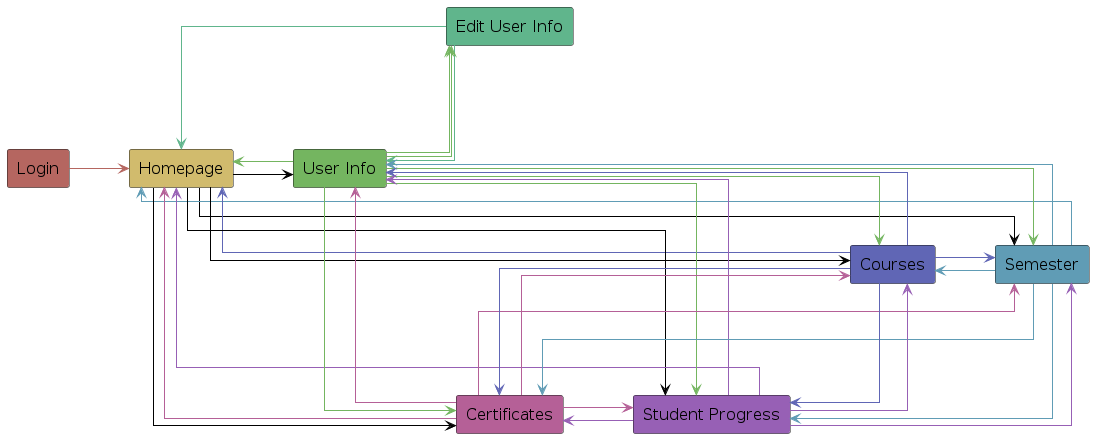
\includegraphics[width=1.0\textwidth]{diagram.png}
    \caption{\gr{Σελίδες και διαδρομές της ιστοσελίδας} ECE-Students}
    \label{fig:enter-label}
\end{figure}

\subsection{\gr{Χρήση της εφαρμογής}}
\gr{Αναλυτικότερα, οι λειτουργίες τις κάθε σελίδας φαίνονται παρακάτω:}

\par
\textbf{Login Page}
\\\gr{Η πρώτη σελίδα που βλέπει ο χρήστης. Από εκεί γίνεται η αυθεντικοποίηση και αποκτά πρόσβαση στην αρχική σελίδα της εφαρμογής. Εάν ο χρήστης είσάγει όνομα χρήστη που δεν υπάρχει στη βάση δεδομένων ή λάθος κωδικό πρόσβασης, ο δρομολογητής εμφανίζει αντίστοιχο μήνυμα λάθους.}

\begin{figure}[H]
    \centering
    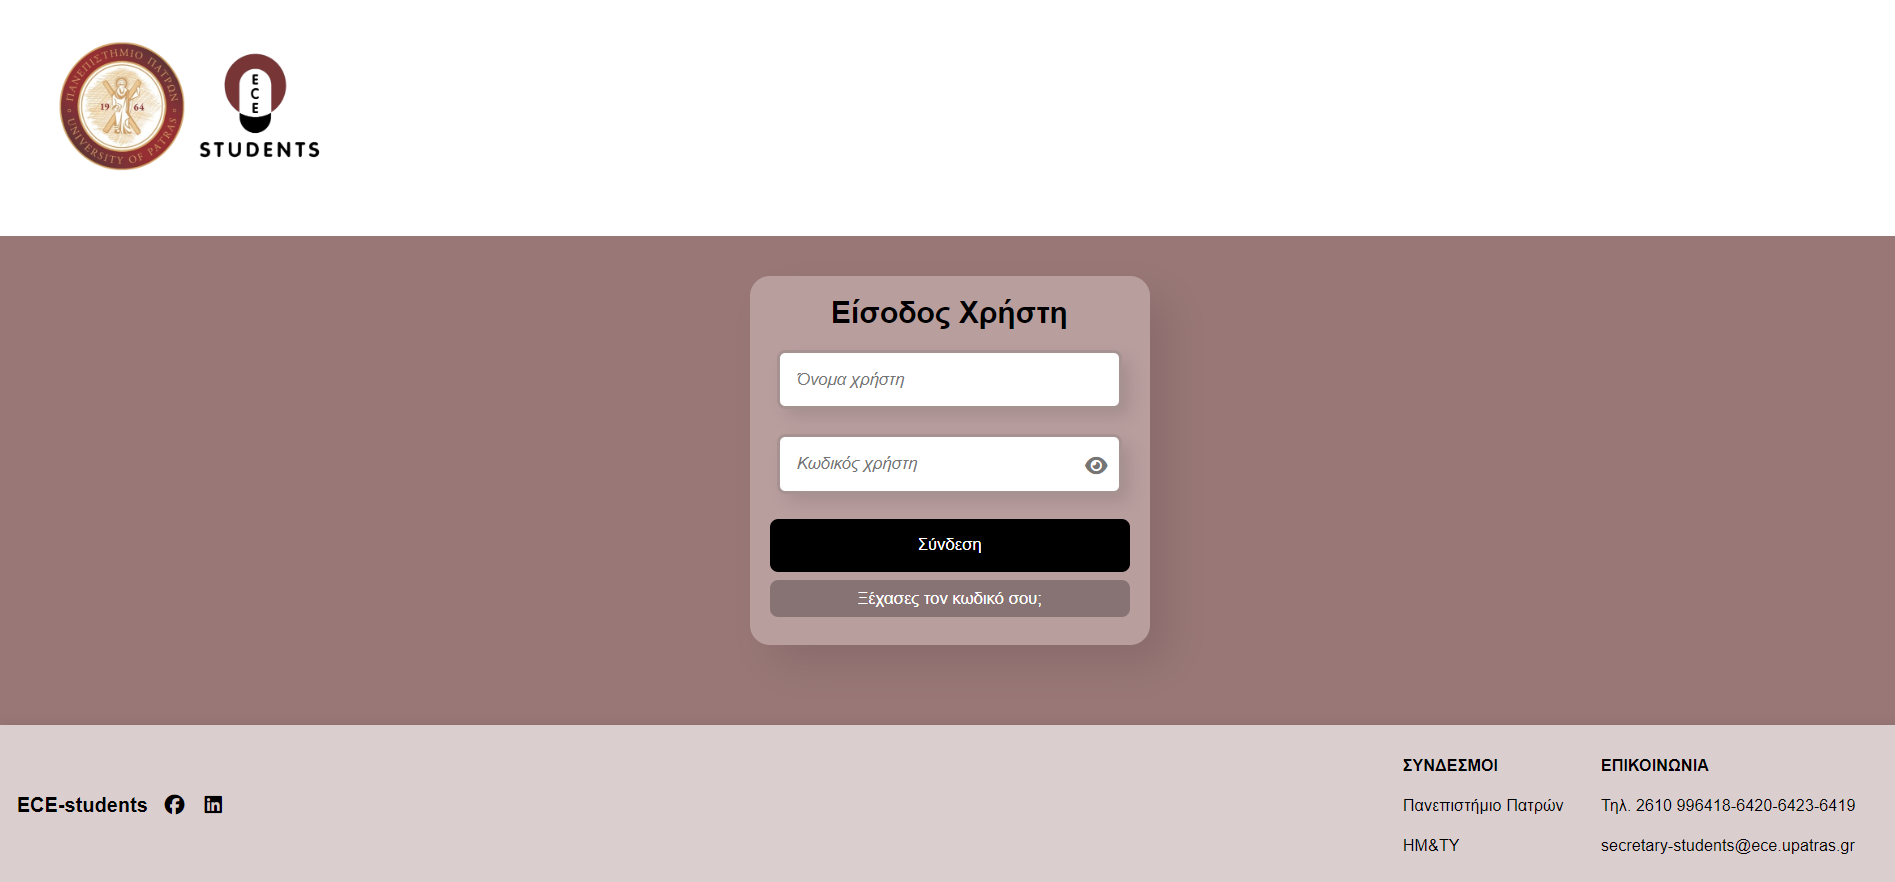
\includegraphics[width=1.0\textwidth]{login.png}
    \caption{Login Page \gr{της ιστοσελίδας} ECE-Students}
    \label{fig:enter-label}
\end{figure}

\begin{figure}[H]
    \centering
    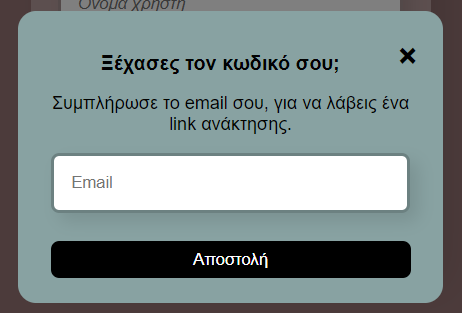
\includegraphics[width=0.4\textwidth]{login_popup.png}
    \caption{Popup \gr{του} Login Page.}
    \label{fig:enter-label}
\end{figure}

\textbf{Home Page}
\\\gr{Η αρχική σελίδα της εφαρμογής. Περιλαμβάνει ένα} container \gr{με ανακοινώσεις και συνδέσμους για άλλες υπηρεσίες του τμήματος. Επίσης, όπως όλες οι σελίδες περιλαμβάνει το} navigation menu \gr{της ιστοσελίδας.}

\begin{figure}[H]
    \centering
    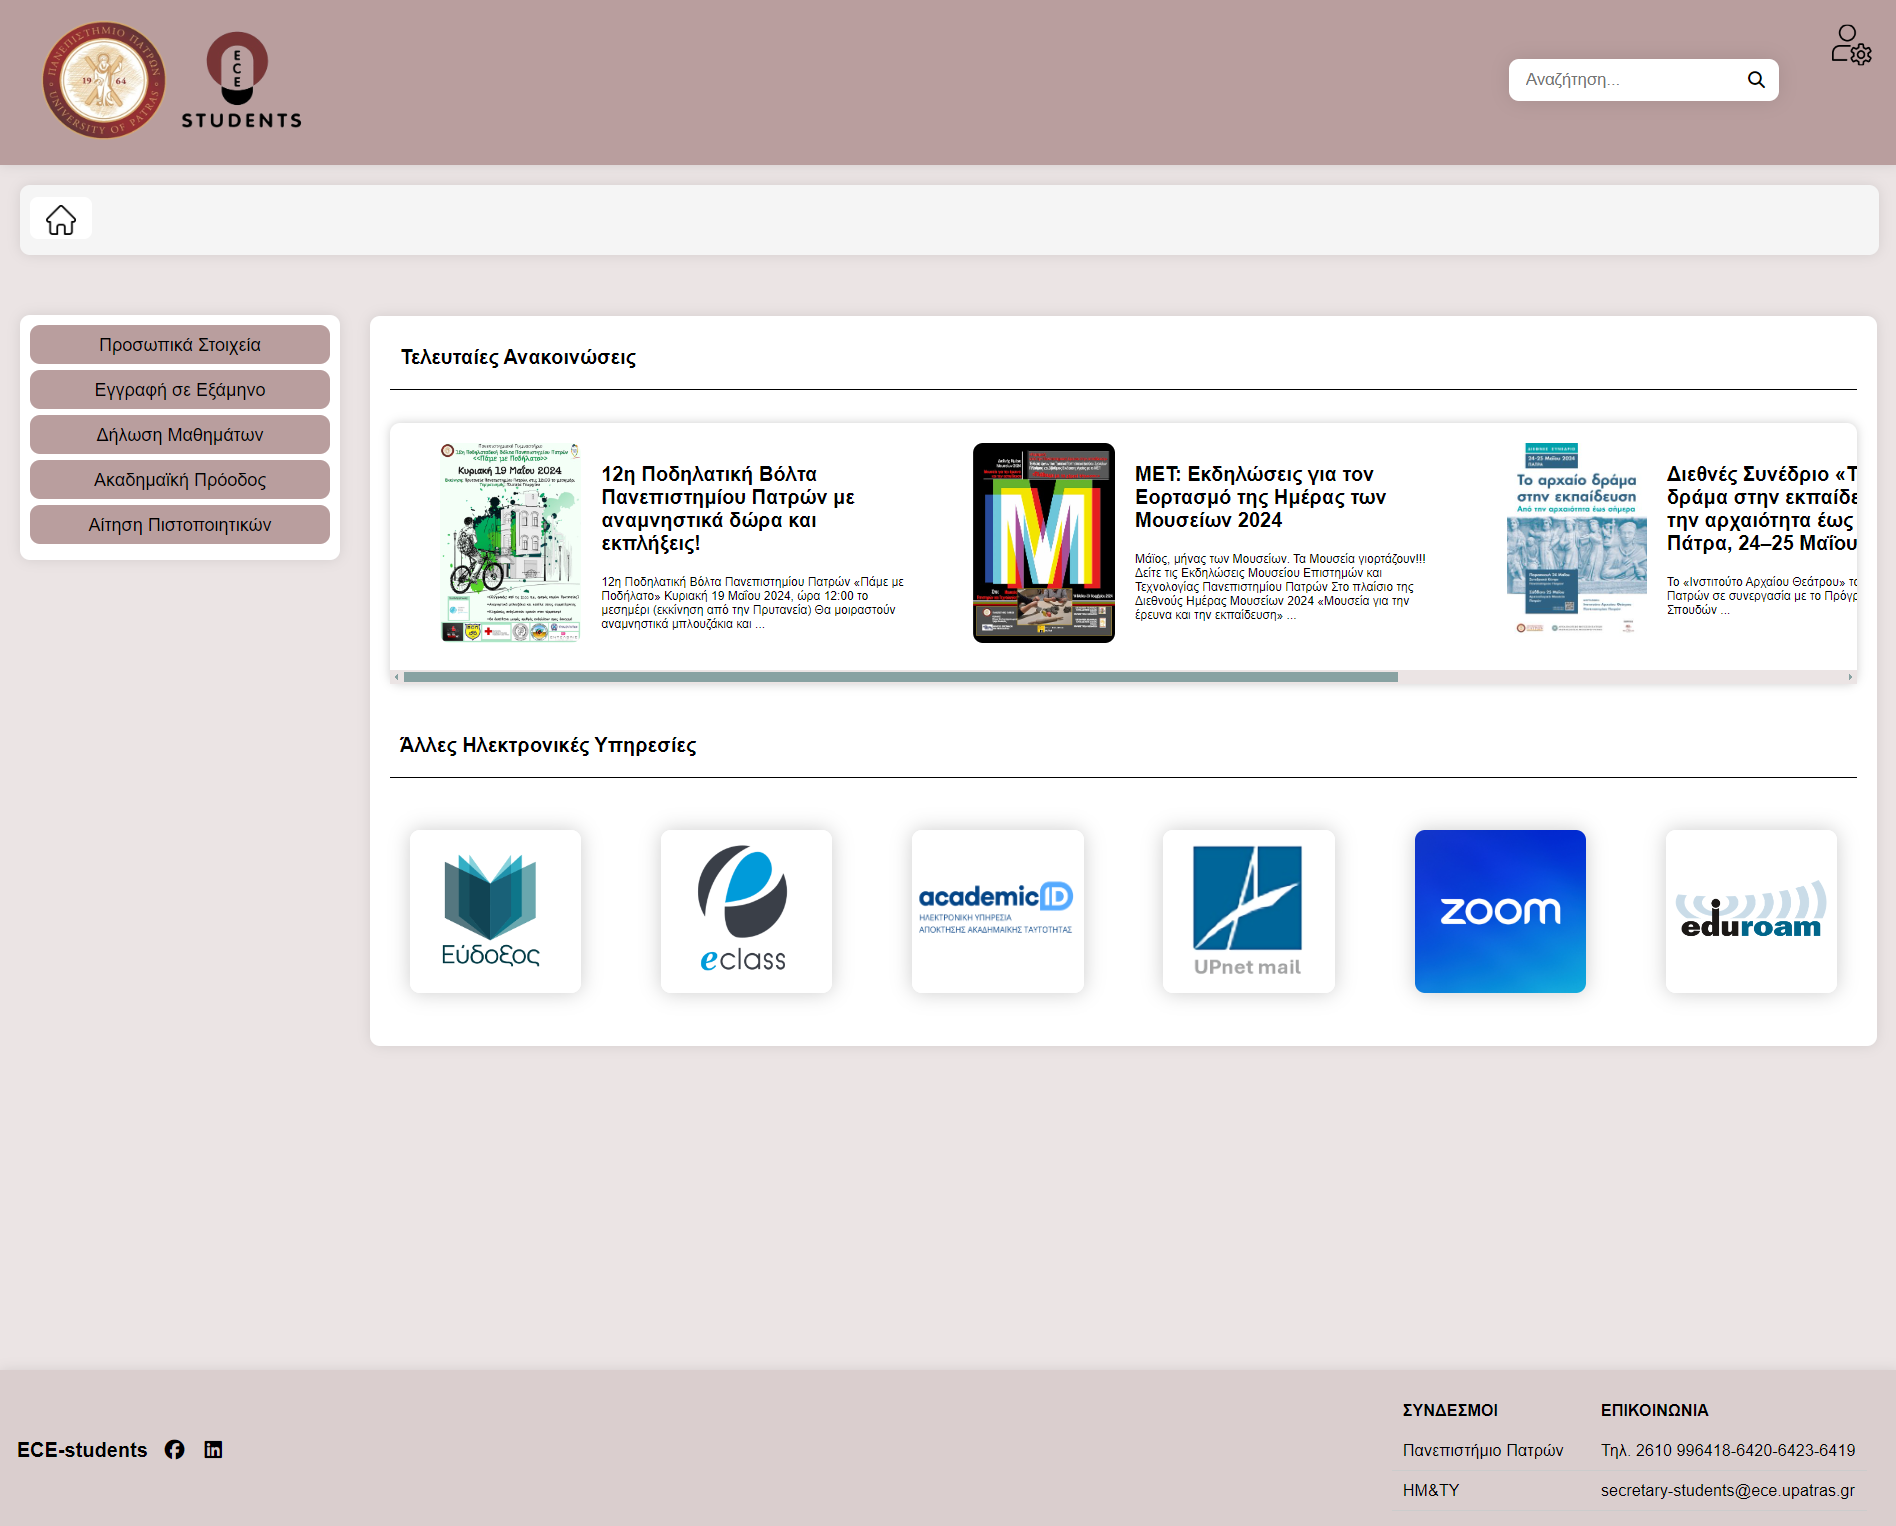
\includegraphics[width=1.0\textwidth]{home_page.png}
    \caption{\gr{Αρχική σελίδα της ιστοσελίδας} ECE-Students}
    \label{fig:enter-label}
\end{figure}

\textbf{User Info Page - Edit User Info Page}
\\\gr{Η σελίδα με τα προσωπικά στοιχεία του χρήστη περιλαμβάνει πίνακα των στοιχείων και ένα κουμπί για επεξεργασία τους που κατευθύνει τον χρήστη στην αντίστοιχη σελίδα,} Edit User Info. \gr{Η σελίδα αυτή περιλαμβάνει την φόρμα επεξεργασίας των στοιχείων.}

\begin{figure}[H]
    \centering
    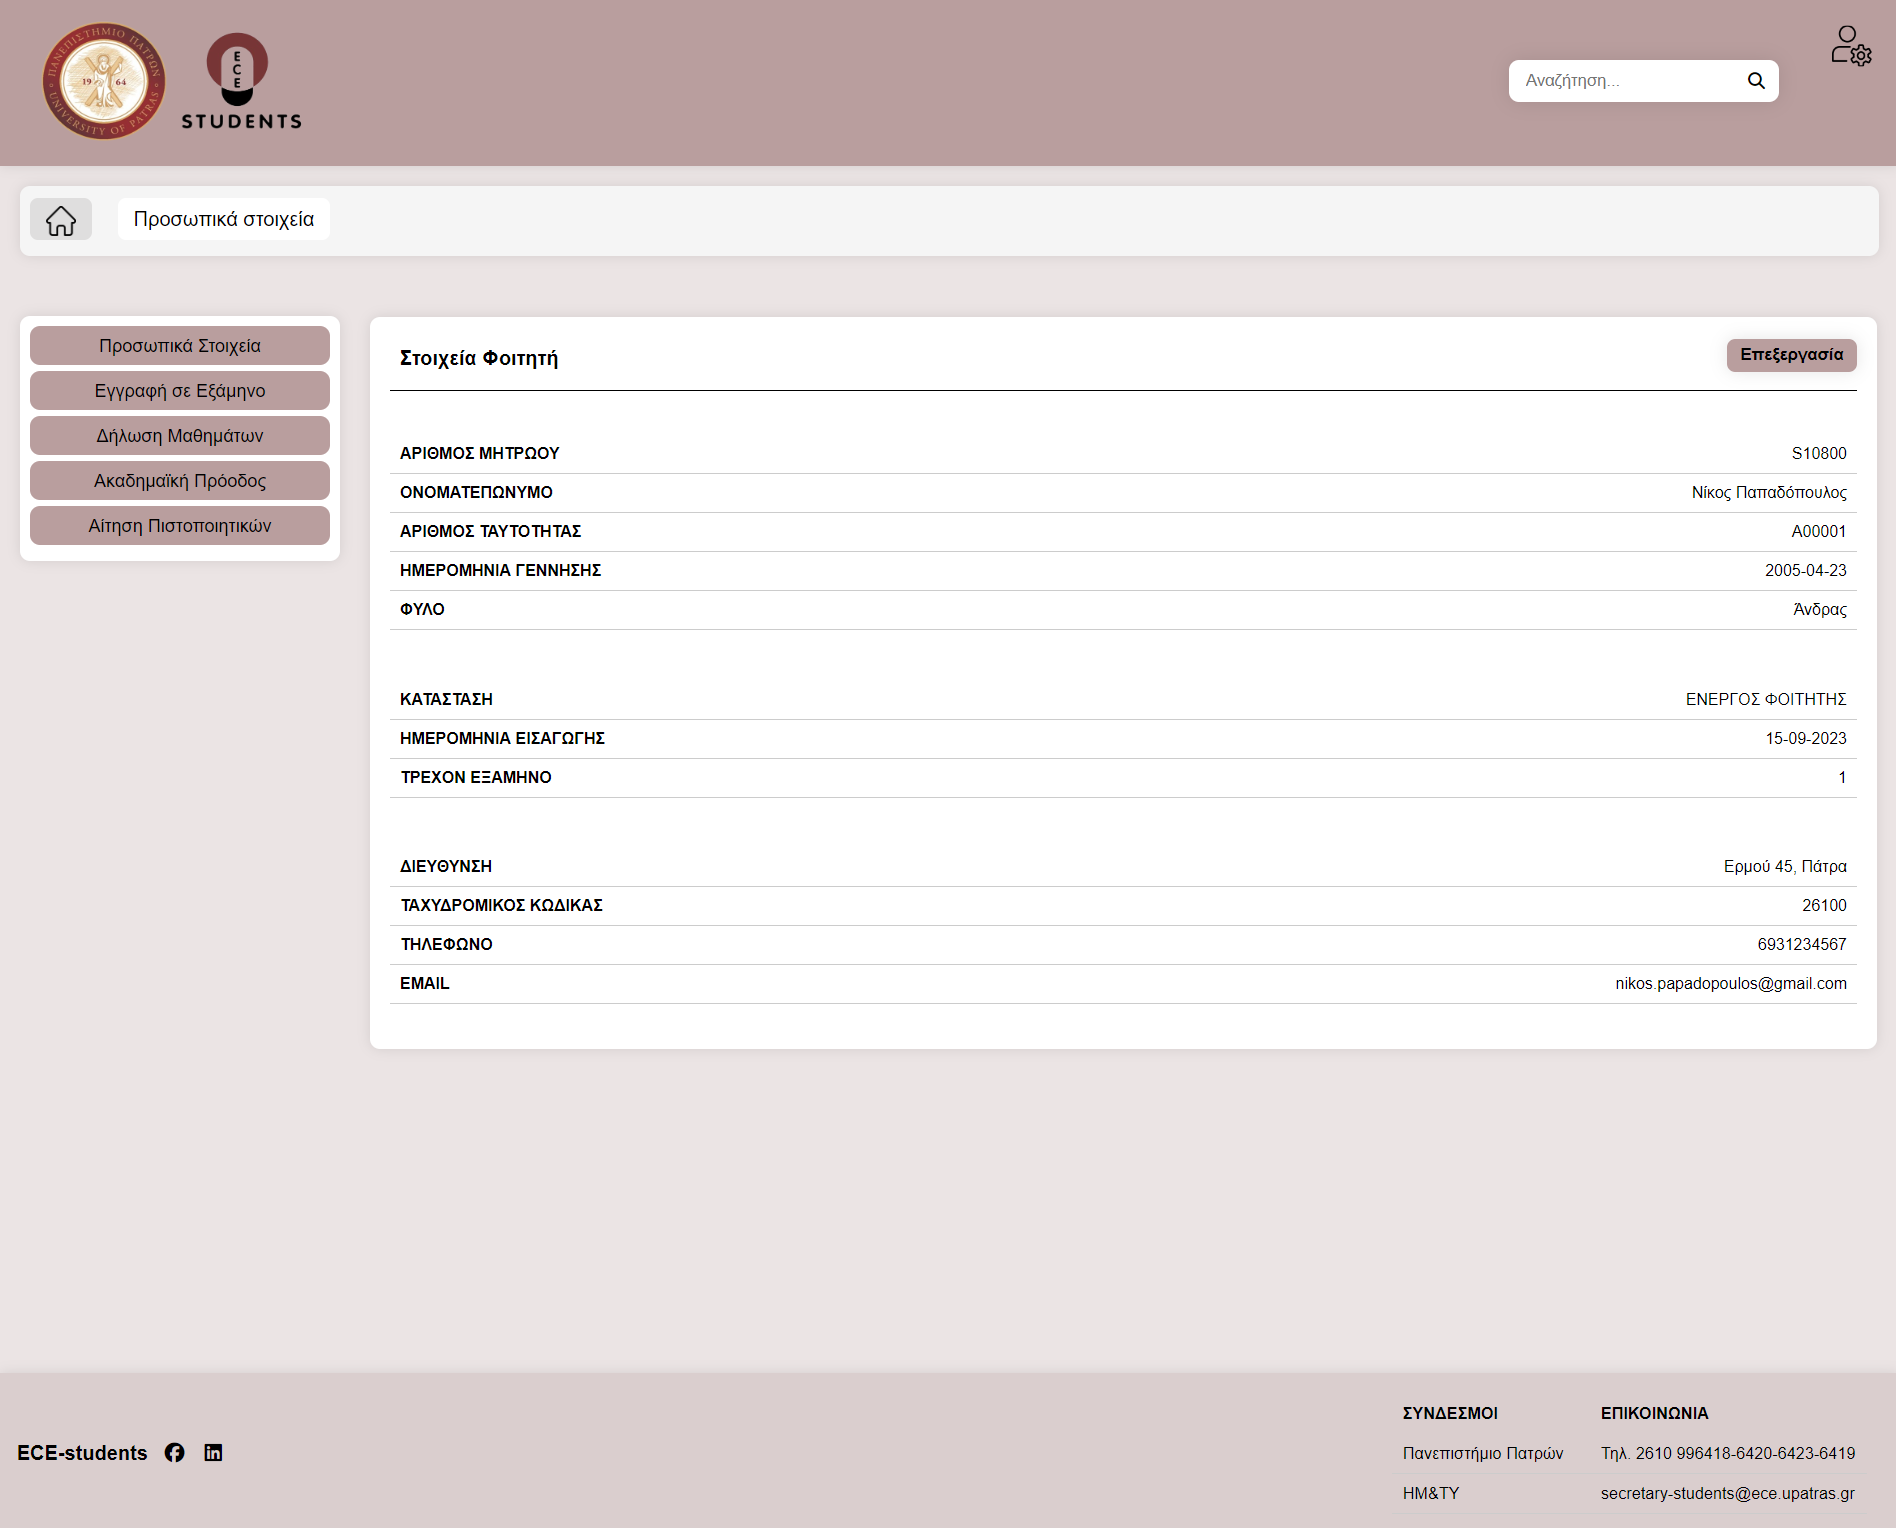
\includegraphics[width=1.0\textwidth]{user_info.png}
    \caption{\gr{Σελίδα προσωπικών στοιχείων χρήστη}}
    \label{fig:enter-label}
\end{figure}

\begin{figure}[H]
    \centering
    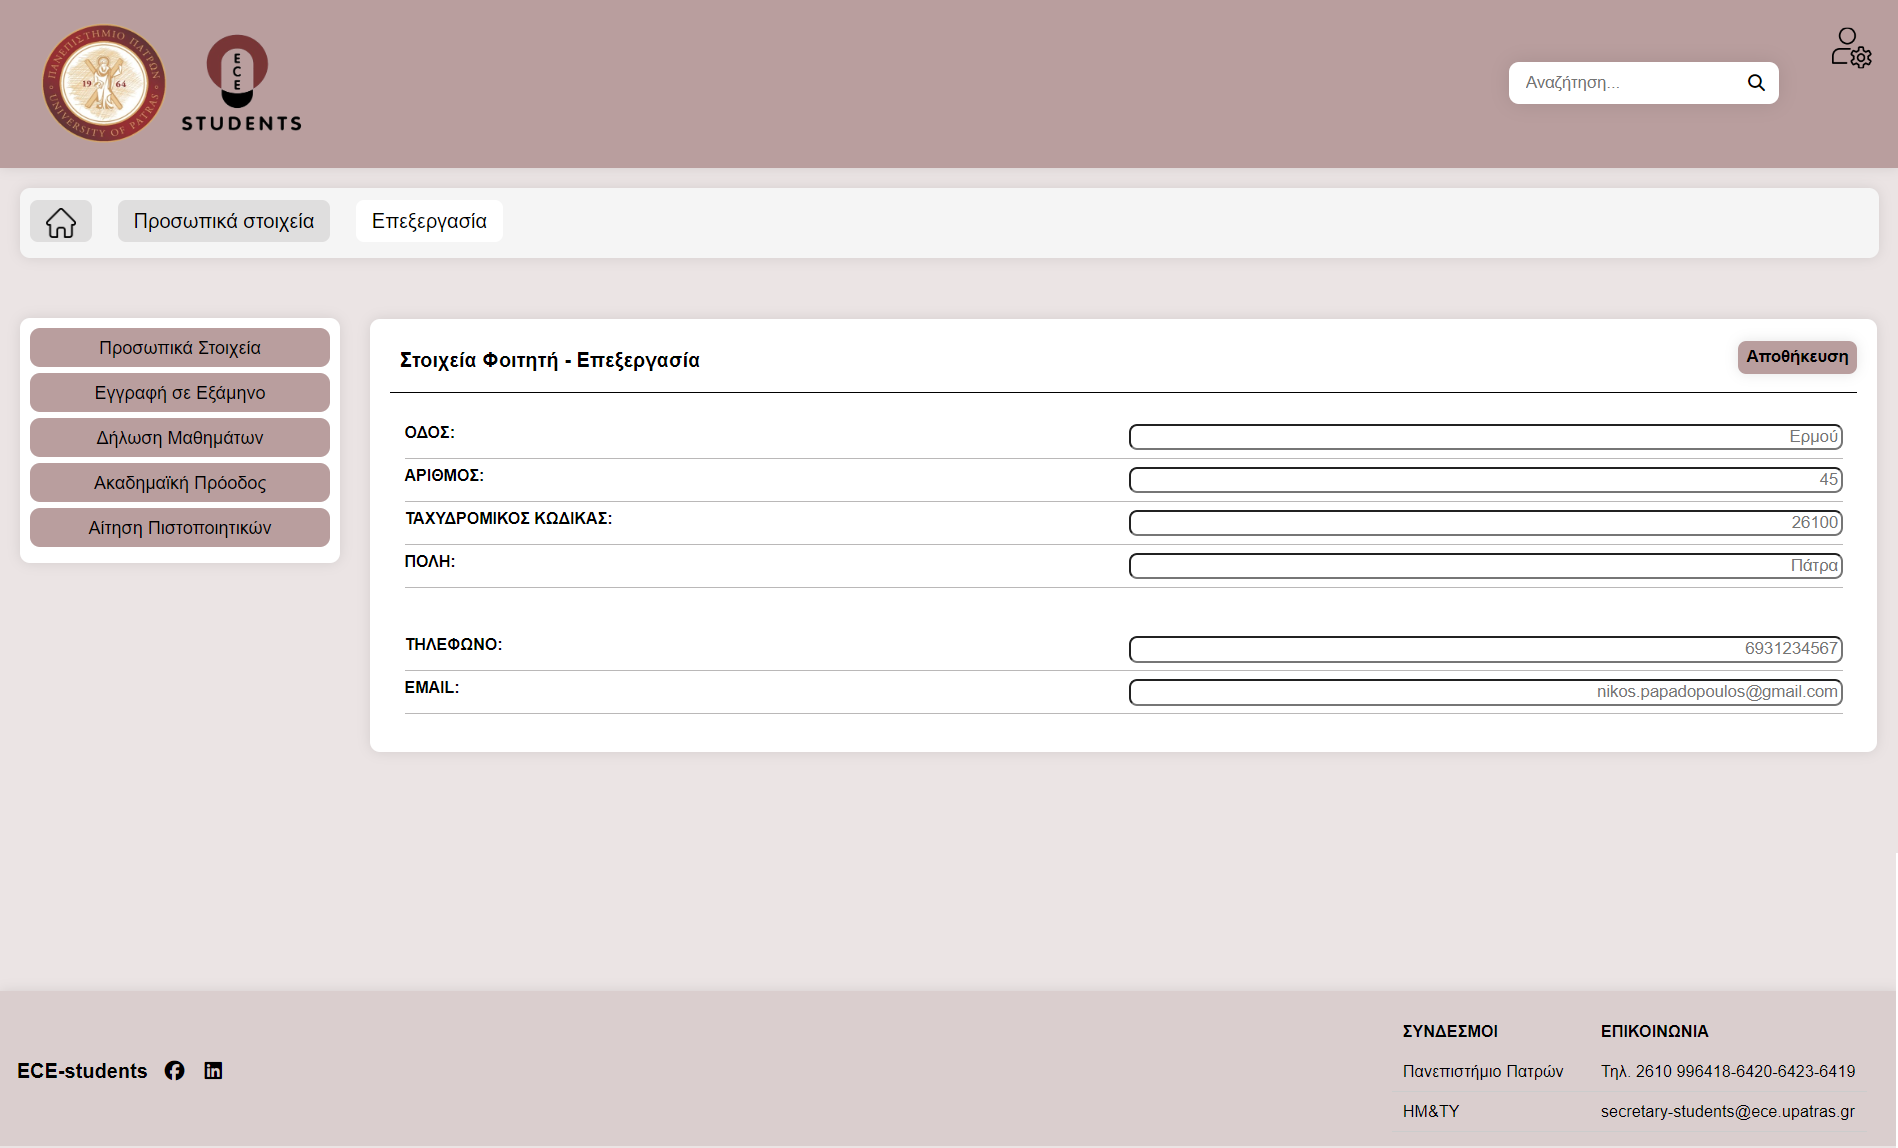
\includegraphics[width=1.0\textwidth]{edit_user_info.png}
    \caption{\gr{Σελίδα επεξεργασίας προσωπικών στοιχείων χρήστη}}
    \label{fig:enter-label}
\end{figure}

\textbf{Semester Page}
\\\gr{Η σελίδα επανεγγραφής σε εξάμηνο περιλαμβάνει στοιχεία της τελευταίας εγγραφής και κουμπί αίτησης επανεγγραφής σε εξάμηνο. Όταν γίνει η εγγραφή εμφανίζεται} popup \gr{με μήνυμα επιτυχίας.}

\begin{figure}[H]
    \centering
    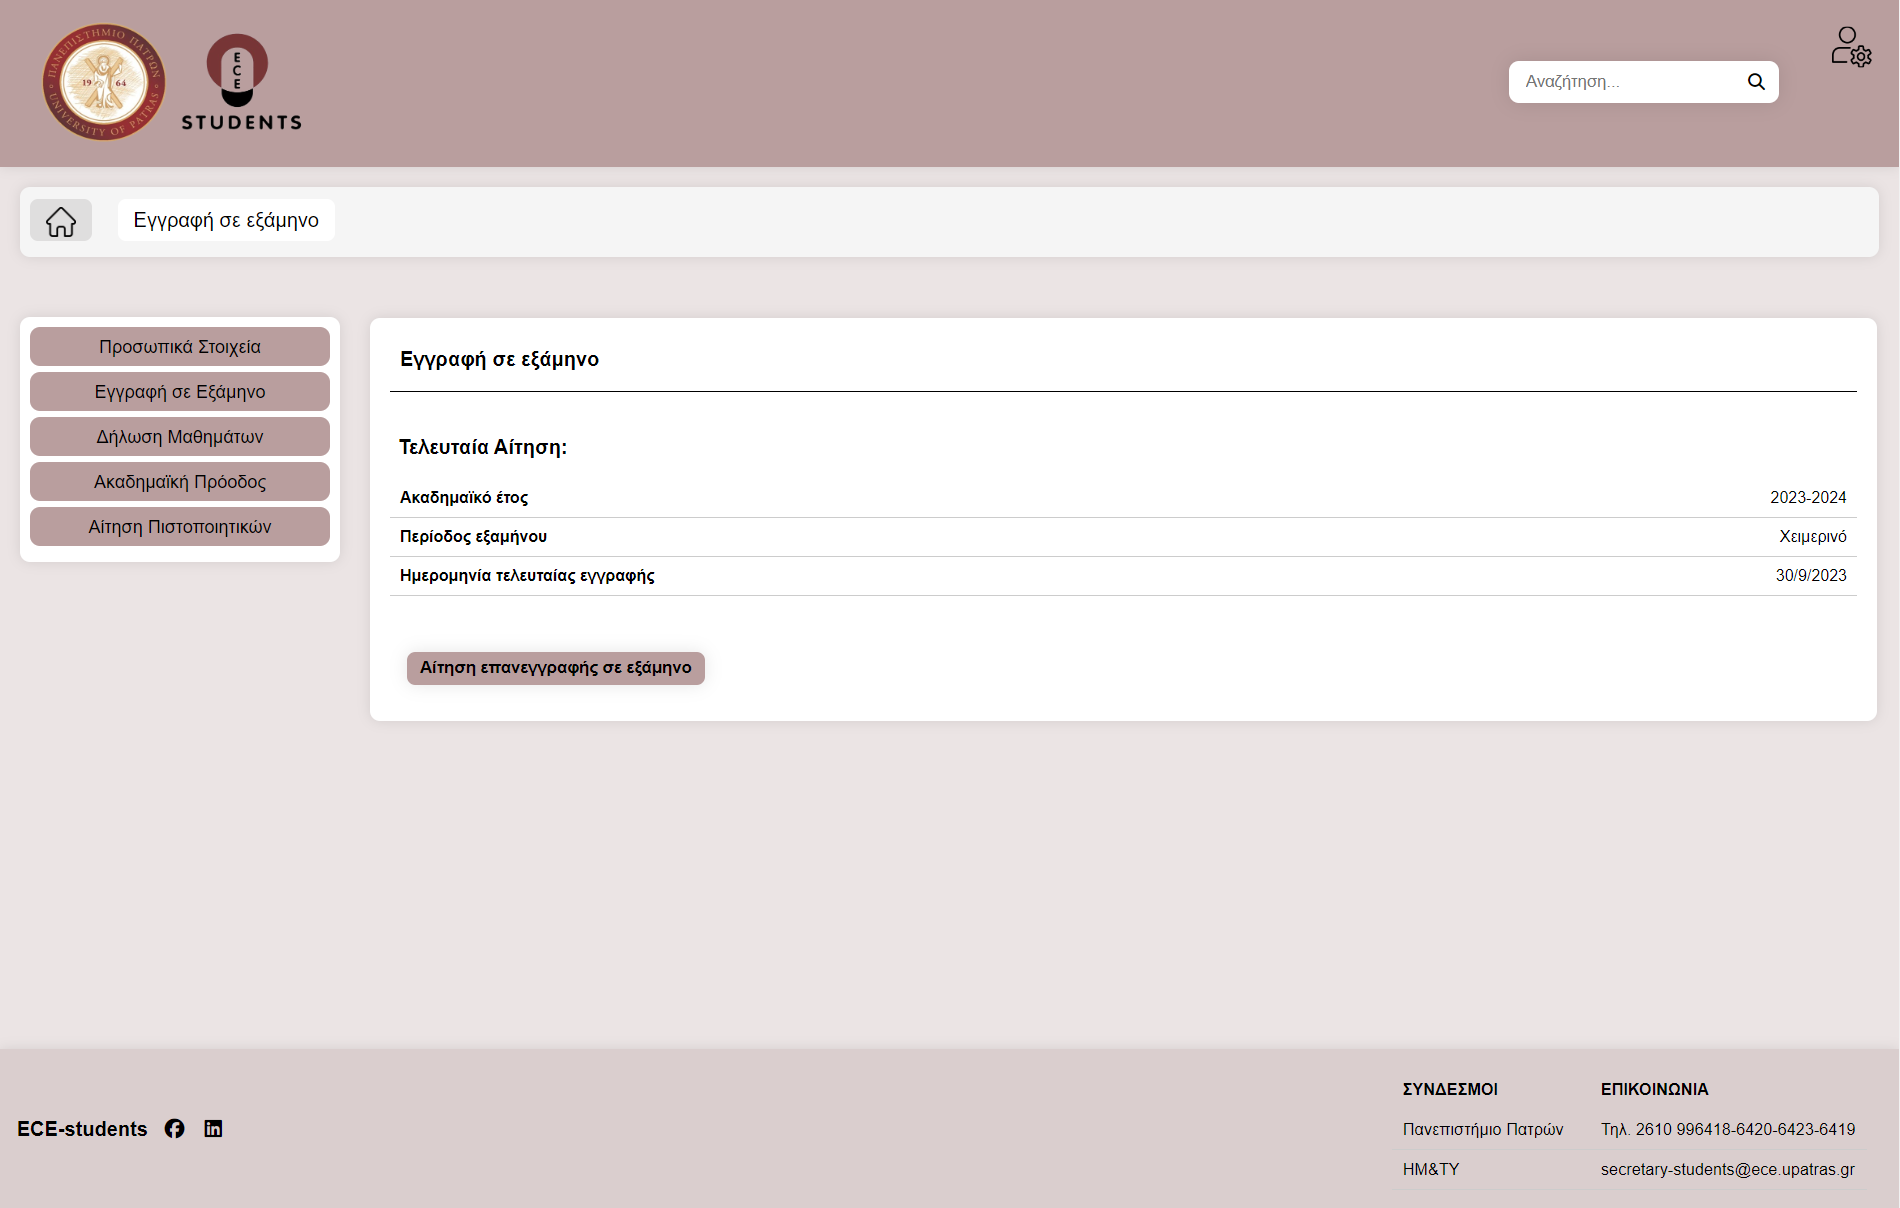
\includegraphics[width=1.0\textwidth]{semester.png}
    \caption{\gr{Σελίδα εγγραφής σε εξάμηνο}}
    \label{fig:enter-label}
\end{figure}

\begin{figure}[H]
    \centering
    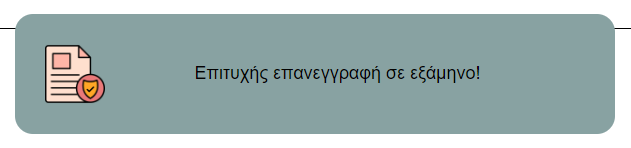
\includegraphics[width=0.4\textwidth]{semester_popup.png}
    \caption{Popup \gr{επιτυχημένης εγγραφής σε εξάμηνο}}
    \label{fig:enter-label}
\end{figure}

\textbf{Courses Page}
\\\gr{Η σελίδα δήλωσης μαθημάτων περιλαμβάνει μια φόρμα για νέα δήλωση ή επεξεργασία παλαιότερης δήλωσης αν έχει ήδη γίνει για το τρέχον εξάμηνο του φοιτητή. Αφού επιλεγεί η δήλωση, εμφανίζεται φόρμα με τα μη επιτυχημένα μαθήματα παλαιότερων εξαμήνων και με τα μαθήματα του τρέχοντος εξαμήνου, για να επηλέξει. Τέλος, εμφανίζεται} popup \gr{επιτυχημένης δήλωσης μαθημάτων.}

\begin{figure}[H]
    \centering
    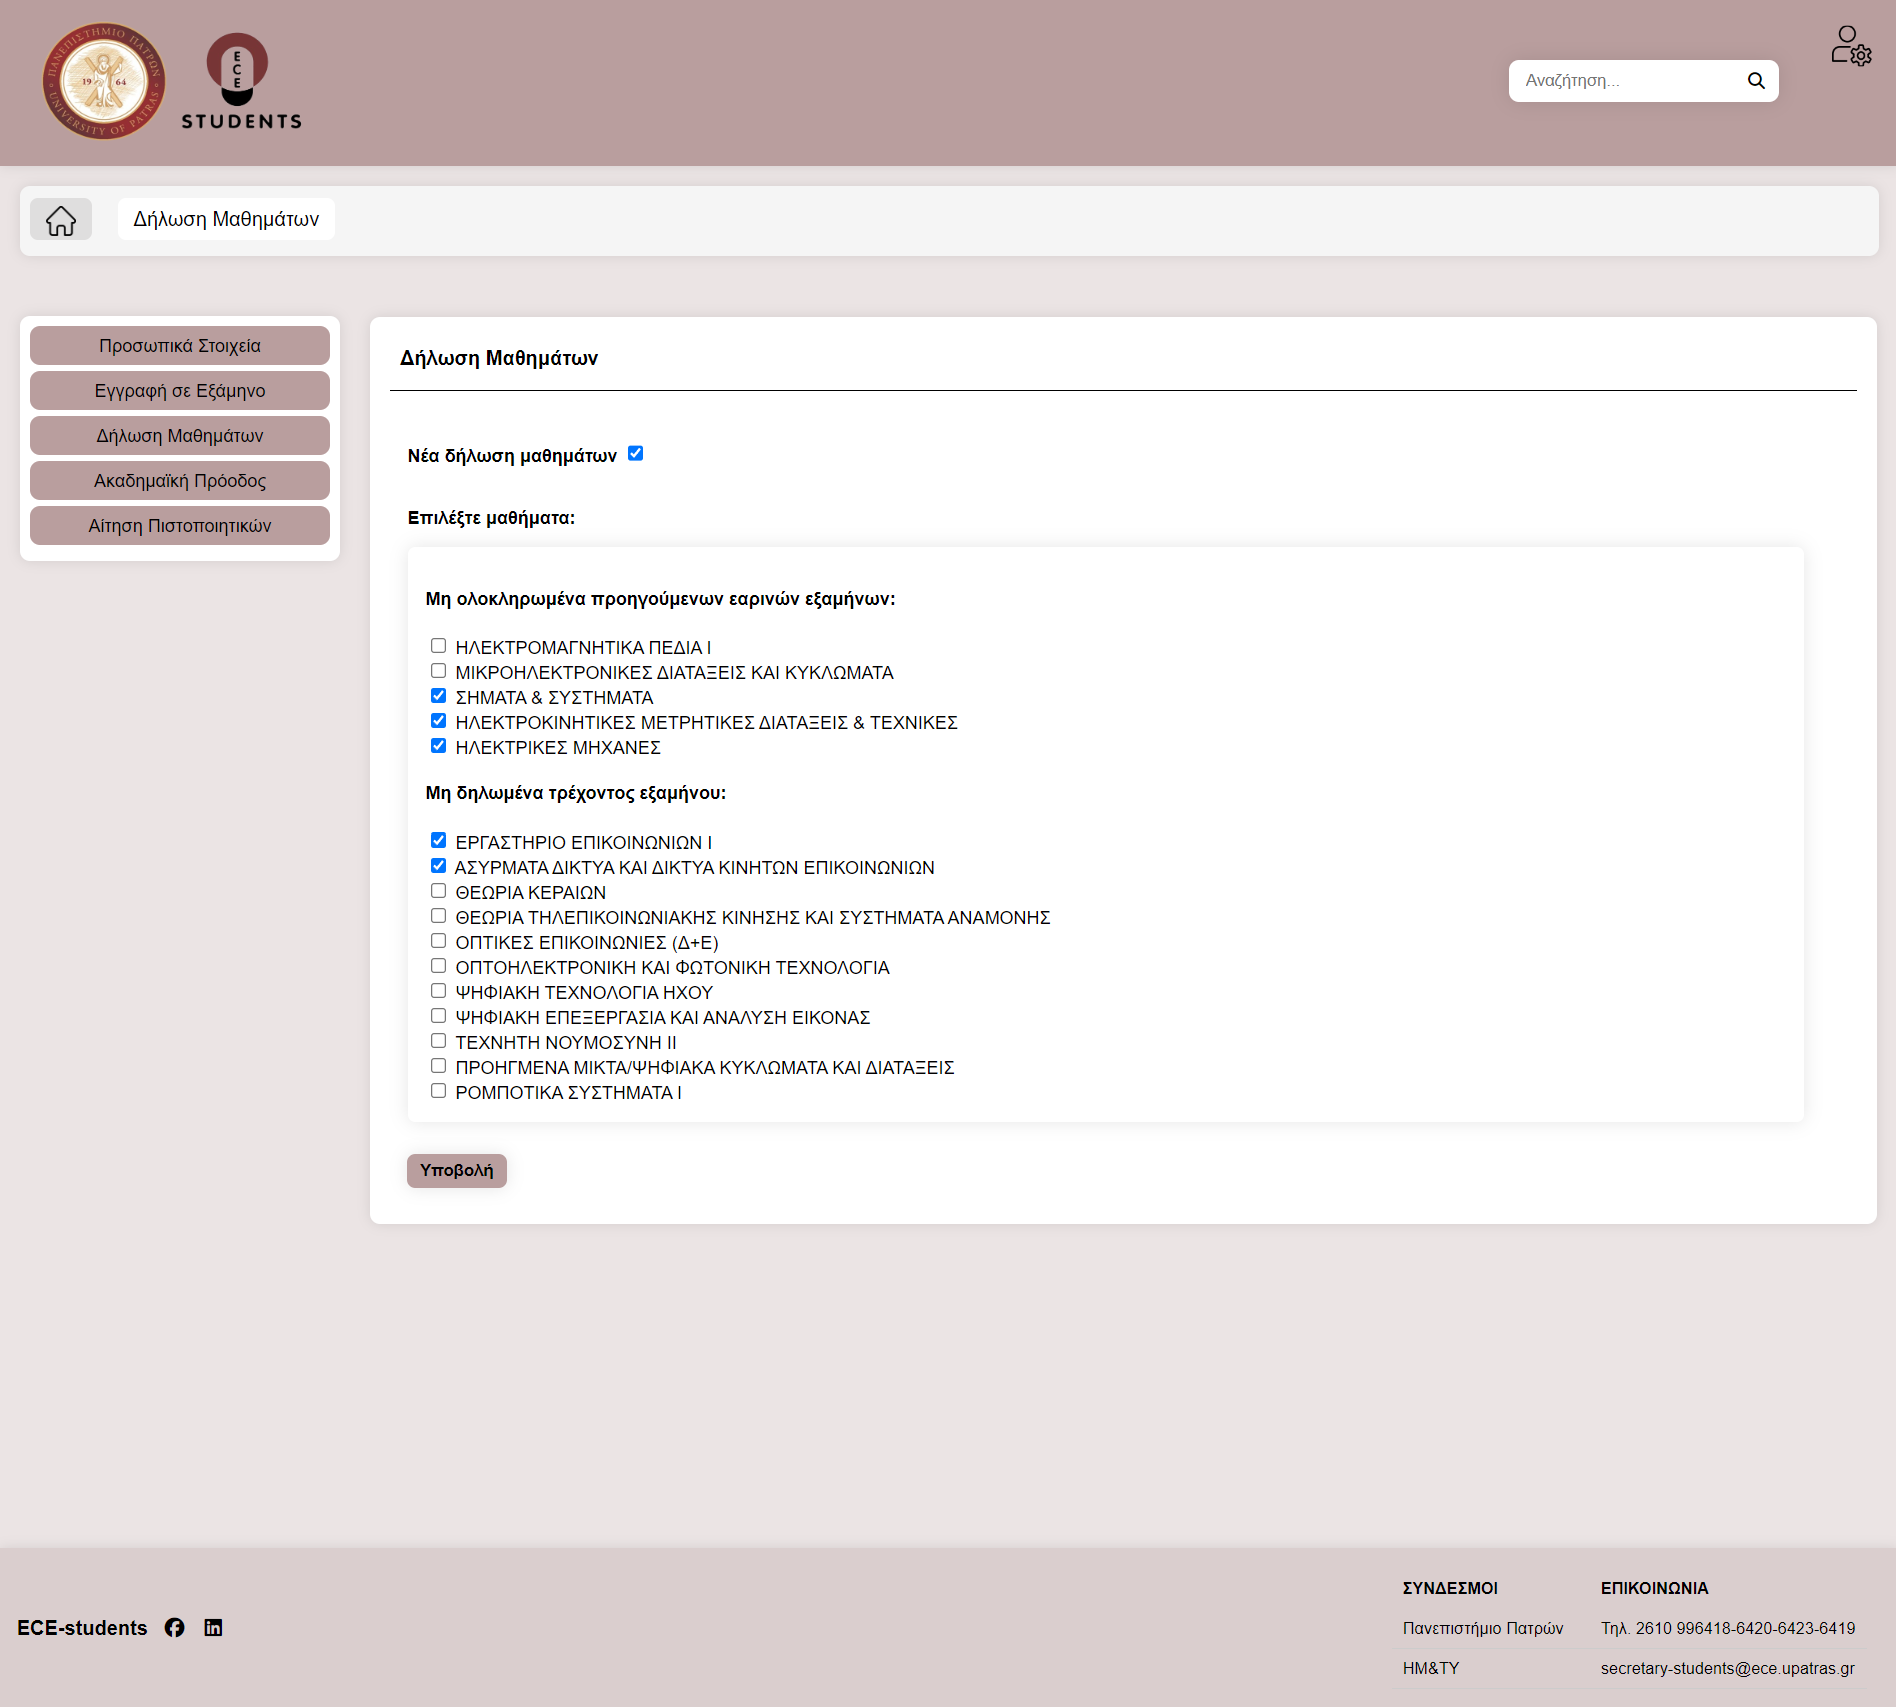
\includegraphics[width=1.0\textwidth]{courses.png}
    \caption{\gr{Σελίδα δήλωσης μαθημάτων με φόρμα δήλωσης}}
    \label{fig:enter-label}
\end{figure}

\begin{figure}[H]
    \centering
    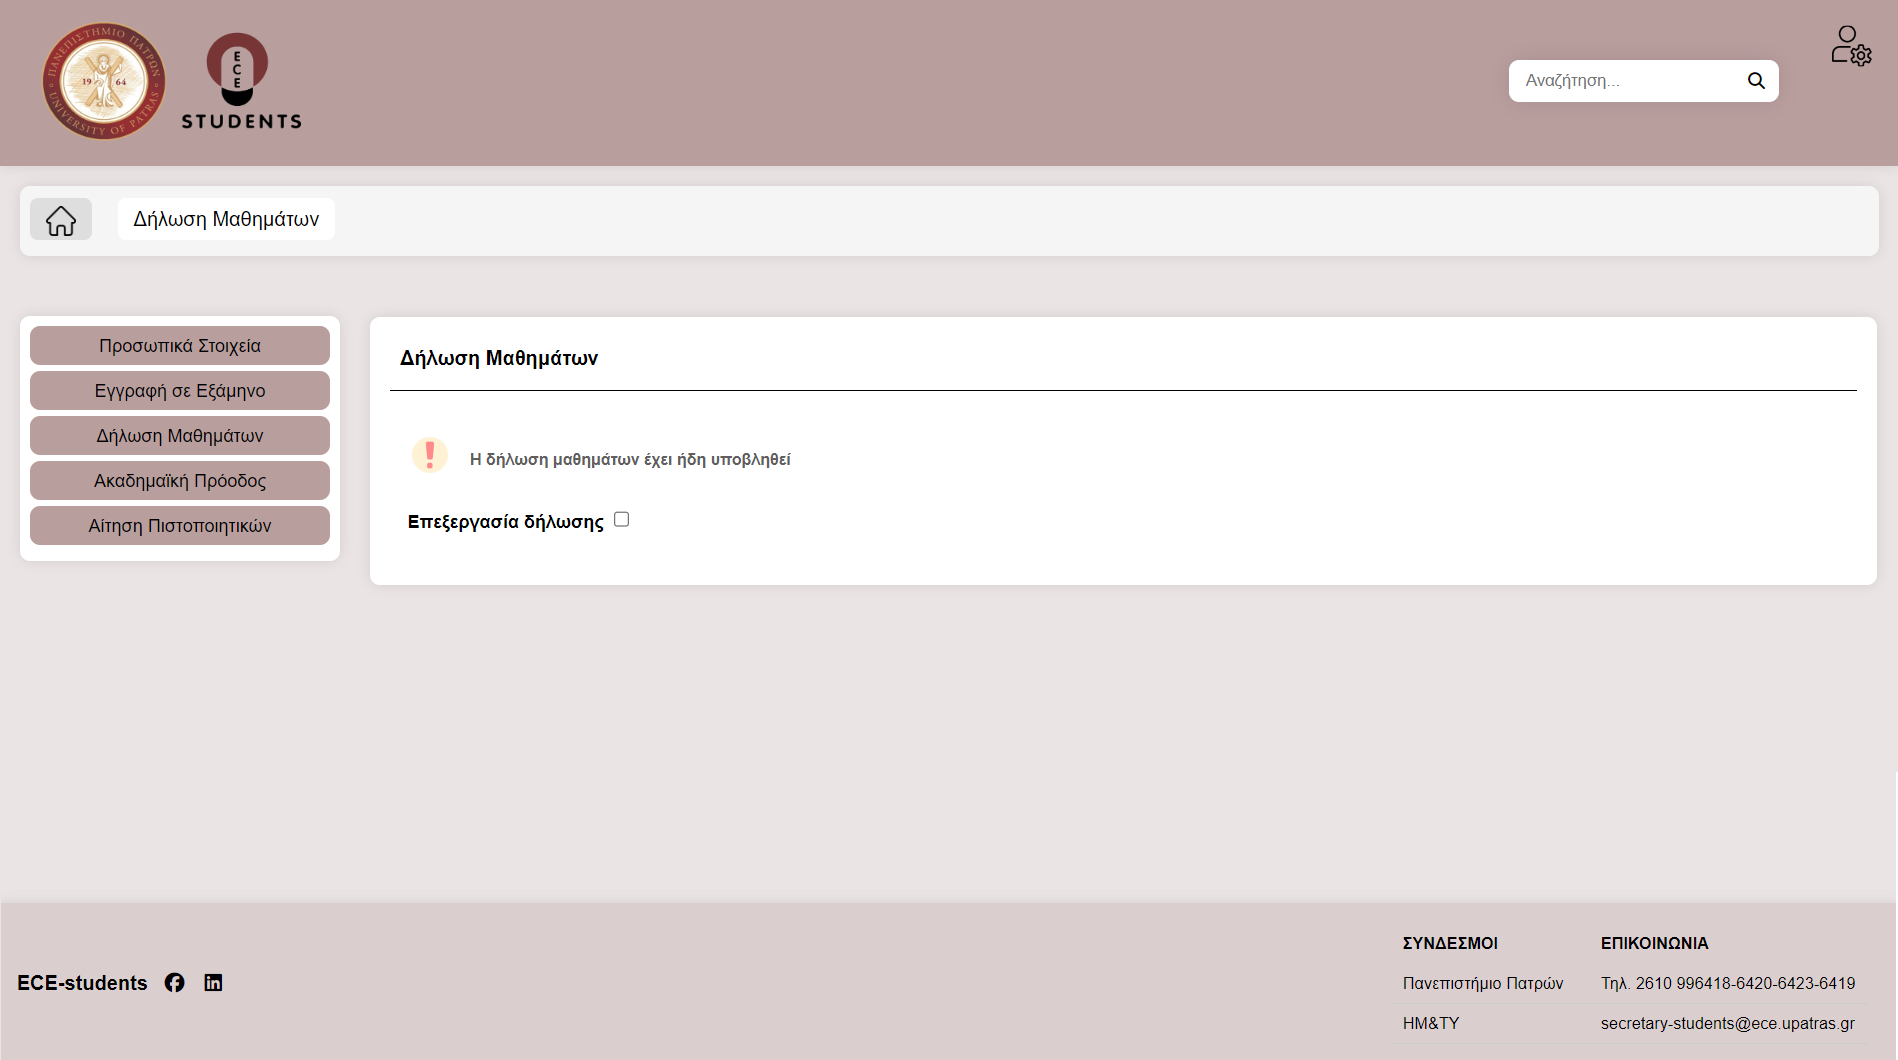
\includegraphics[width=1.0\textwidth]{courses_2.png}
    \caption{\gr{Σελίδα δήλωσης μαθημάτων με επεξεργασία δήλωσης}}
    \label{fig:enter-label}
\end{figure}

\textbf{Student Progress Page}
\\\gr{Η σελίδα της ακαδημαϊκής προόδου του φοιτητή περιλαμβάνει έναν πίνακα με την κατάσταση όλων των μαθημάτων του έως τώρα και τον μέσο όρο του φοιτητή. Με κόκκινο χρώμα αναγράφονται τα μαθήματα με μη προβιβάσιμο βαθμό ή μη συμμετοχής του φοιτητή στην αντίστοιχη εξέταση, ενώ με παύλες τα μαθήματα που δήλωσε στο τελευταίο εξάμηνο εγγραφής και δεν έχουν ακόμα βαθμό. Στη στήλη "έτος" αναγράφεται το έτος τελευταίας δήλωσης του μαθήματος. Ο μέσος όρος υπολογίζεται πολλαπλασσιάζοντας το βαθμό κάθε μαθήματος με το συντελεστή βαρύτητάς του και το άθροισμα των επιμέρους γινομένων διαιρείται με το άθροισμα των συντελεστών βαρύτητας όλων των μαθημάτων.}

\begin{figure}[H]
    \centering
    \includegraphics[width=0.6\textwidth]{progress_all.png}
    \caption{\gr{Σελίδα ακαδημαϊκής προόδου φοιτητή}}
    \label{fig:enter-label}
\end{figure}

\textbf{Certificates Page}
\\\gr{Η σελίδα αίτησης πιστοποιητικών περιλαμβάνει το ιστορικό αιτήσεων του φοιτητή και δυνατότητα νέας αίτησης μέσω φόρμας. Ο φοιτητής μπορεί να κατεβάσει το πιστοποιητικό κάνοντας} click \gr{στον τίτλο του.}

\begin{figure}[H]
    \centering
    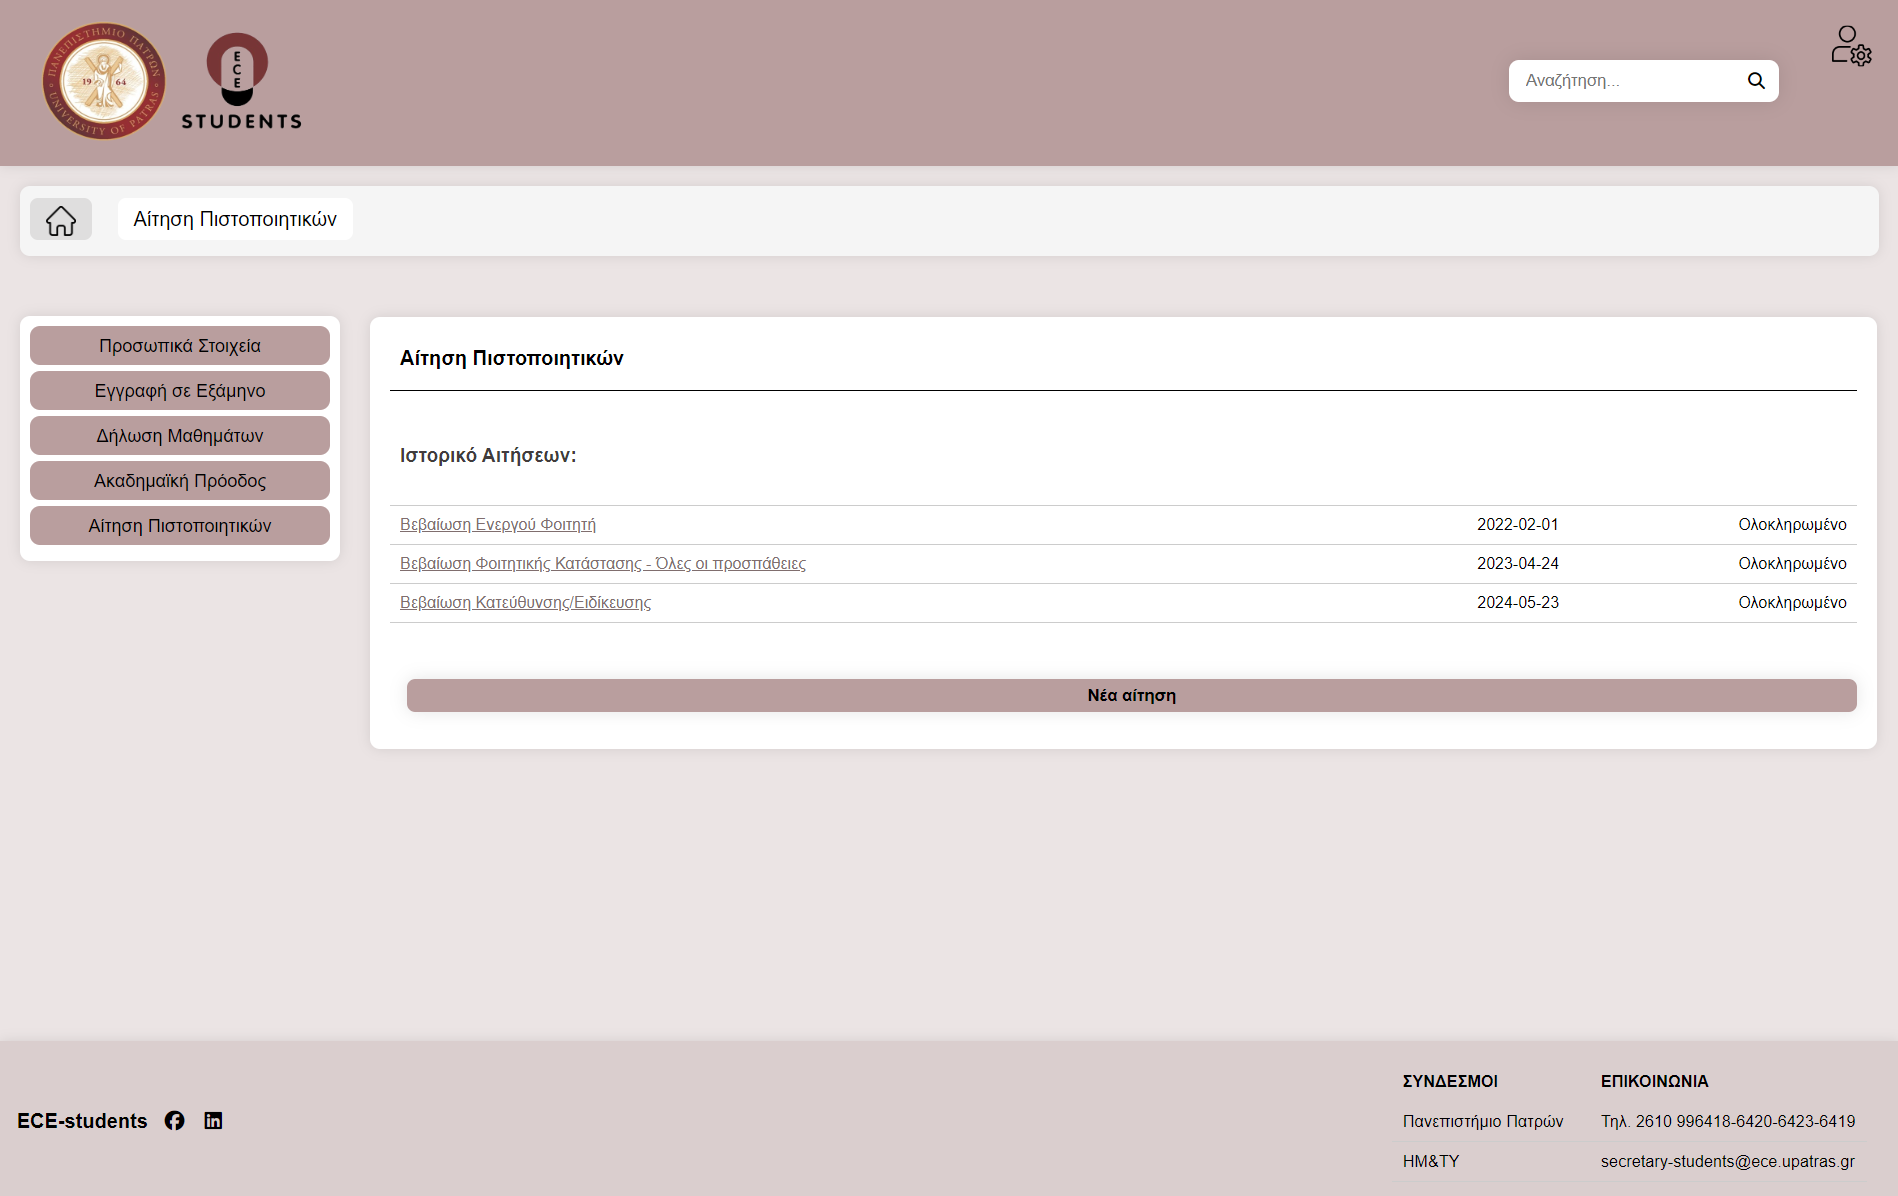
\includegraphics[width=1.0\textwidth]{certificates.png}
    \caption{\gr{Σελίδα αίτησης πιστοποιητικών - Ιστορικό}}
    \label{fig:enter-label}
\end{figure}

\begin{figure}[H]
    \centering
    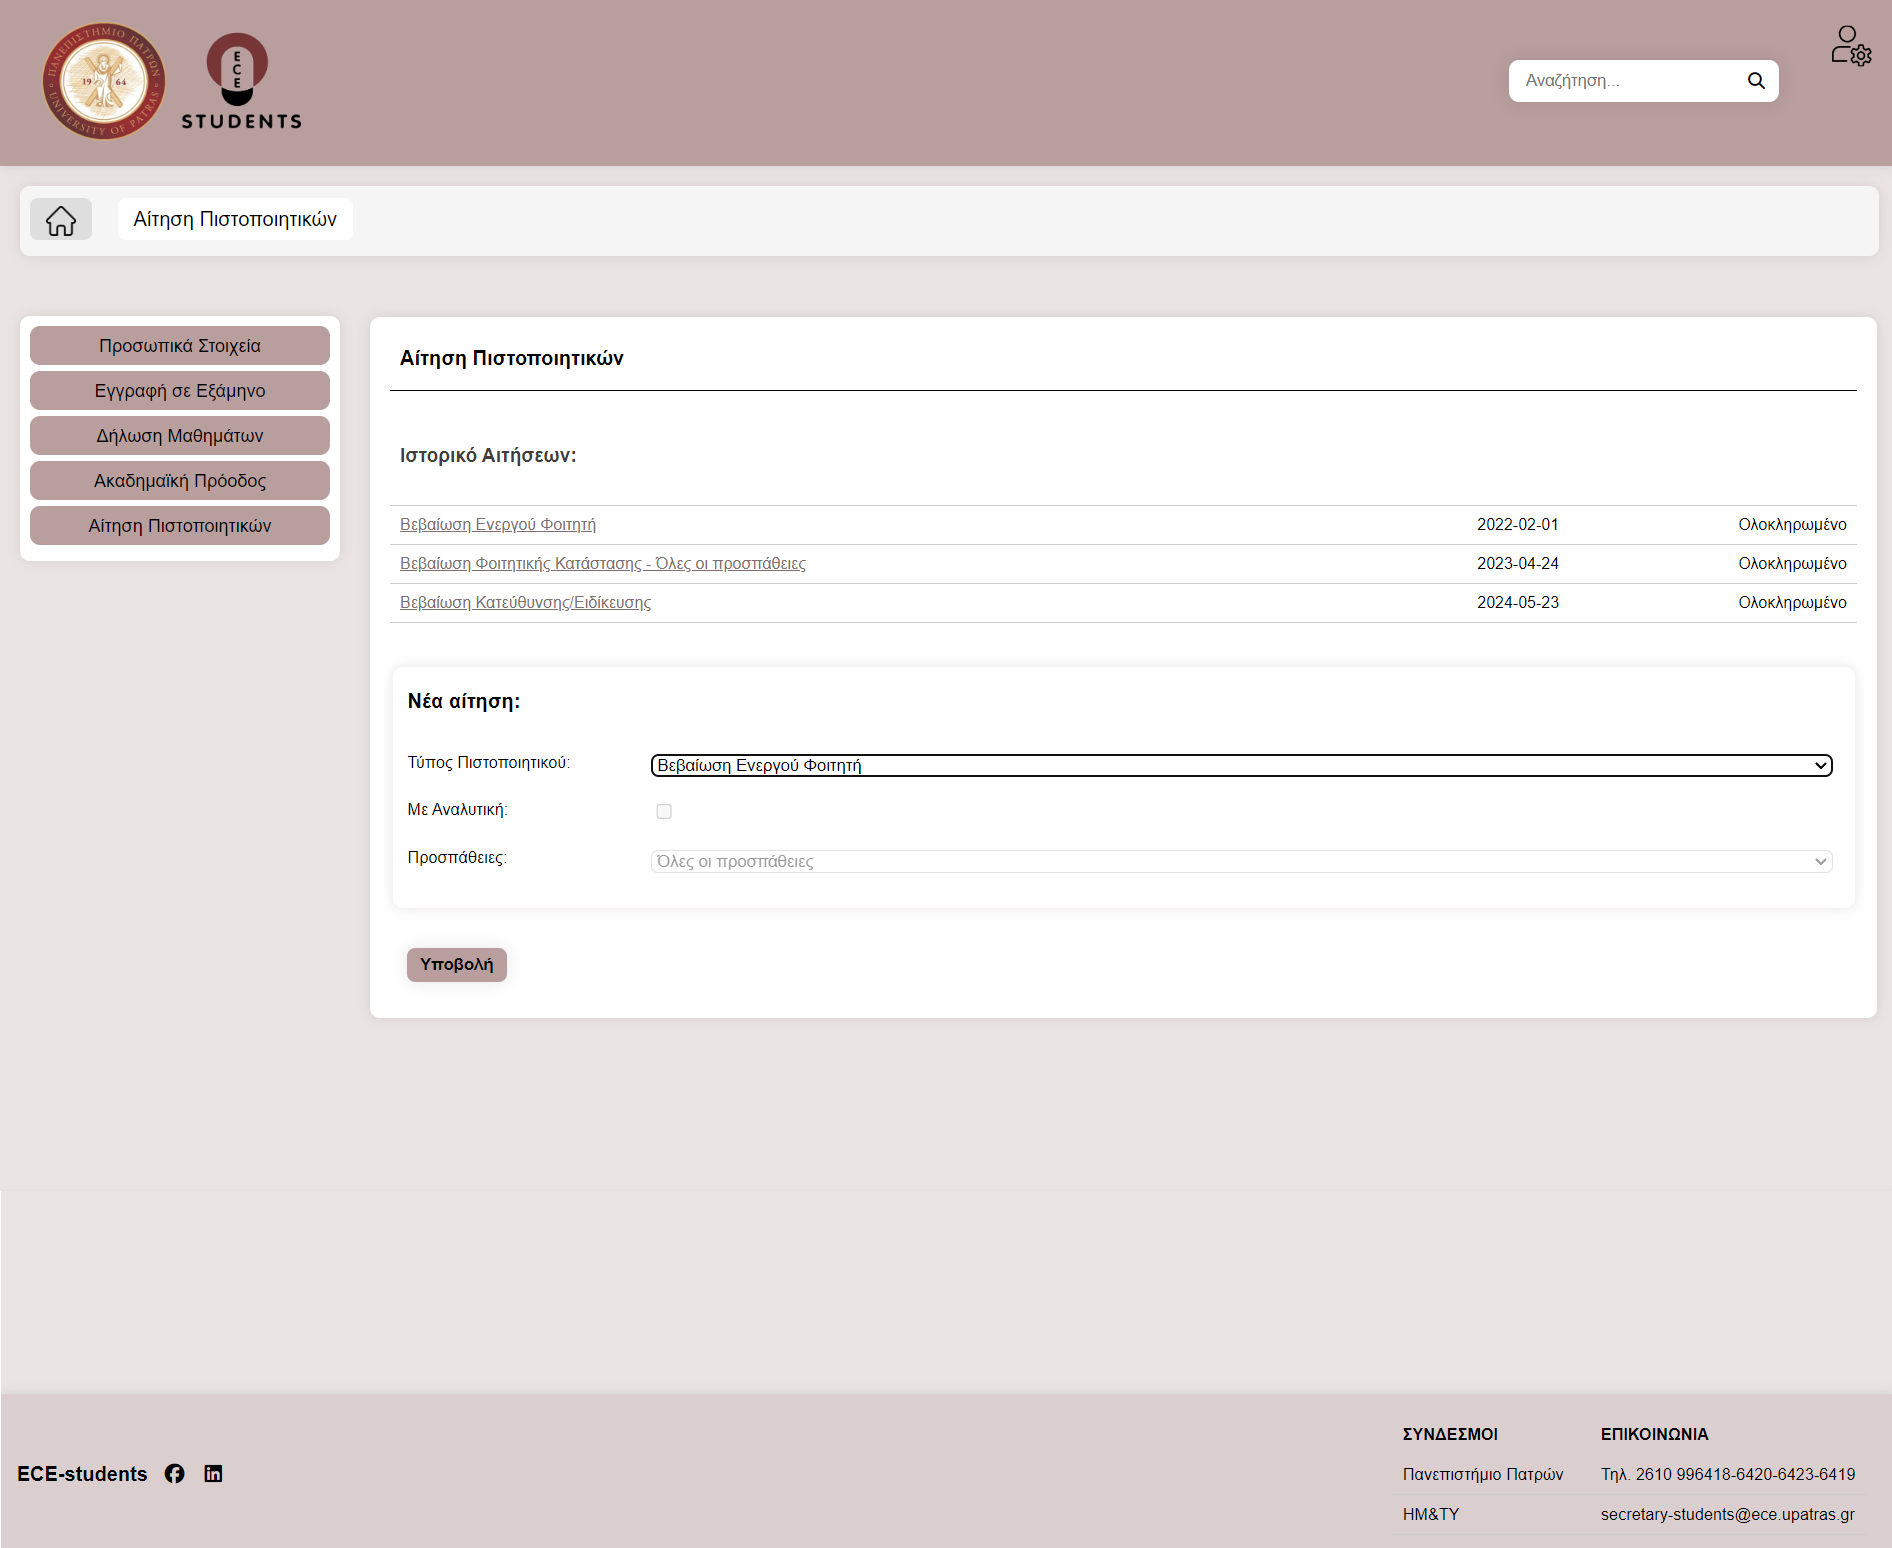
\includegraphics[width=1.0\textwidth]{certificates_form.png}
    \caption{\gr{Σελίδα αίτησης πιστοποιητικών - Φόρμα νέας αίτησης}}
    \label{fig:enter-label}
\end{figure}

\gr{Τέλος, ο χρήστης μπορεί από κάθε σελίδα να κάνει αποσύνδεση.}

\begin{figure}[H]
    \centering
    
\includegraphics[width=0.3\textwidth]{logout.png}
    \caption{\gr{Κουμπί αποσύνδεσης από την ιστοσελίδα}}
    \label{fig:enter-label}
\end{figure}

\gr{Κάποια παραδείγματα σελίδων σε} mobile view:

\begin{figure}[H]
    \centering
    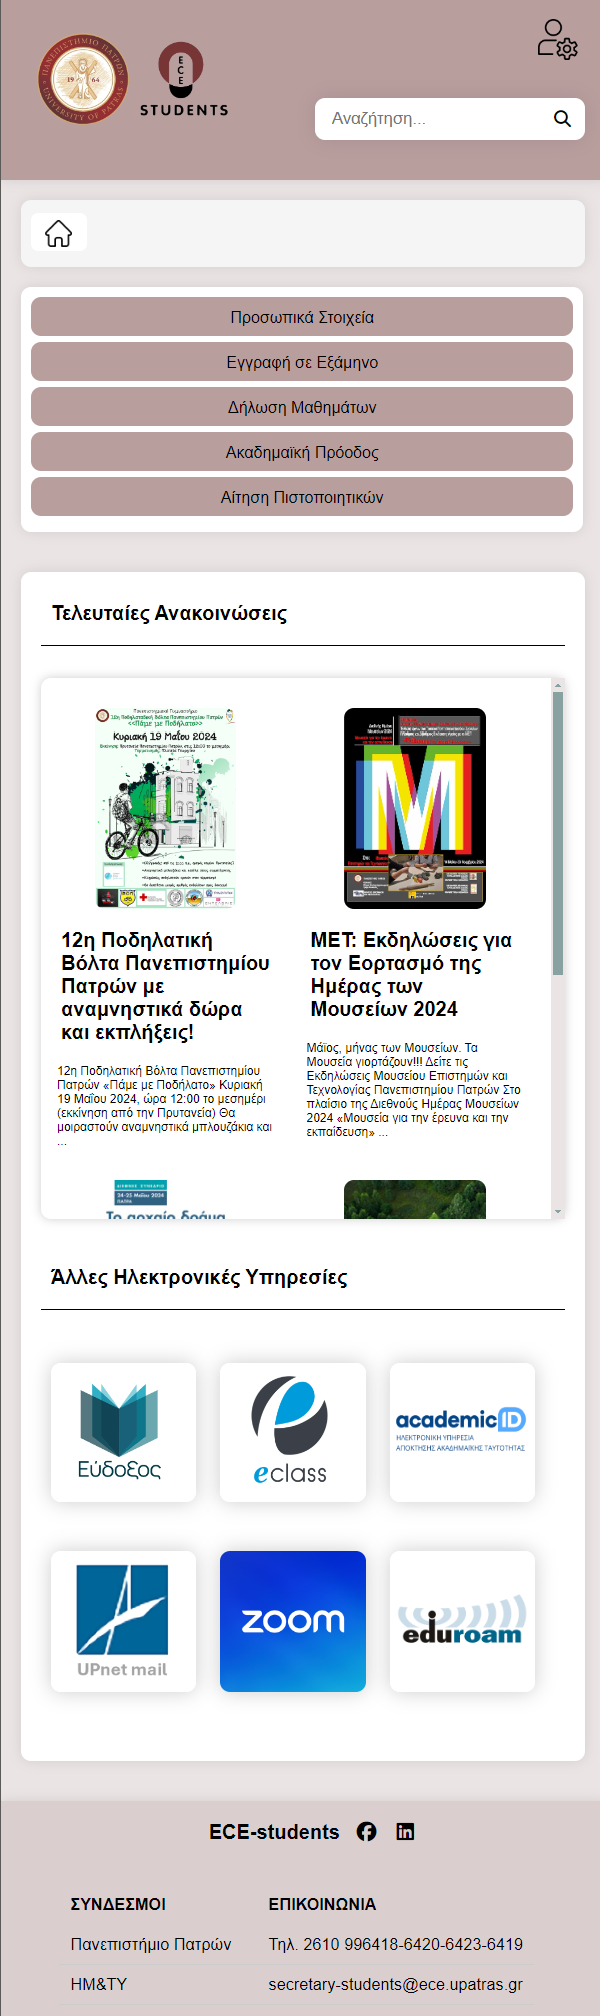
\includegraphics[width=0.3\textwidth]{home_mobile.png}
    \caption{\gr{Αρχική σελίδα σε} mobile view}
    \label{fig:enter-label}
\end{figure}

\begin{figure}[H]
    \centering
    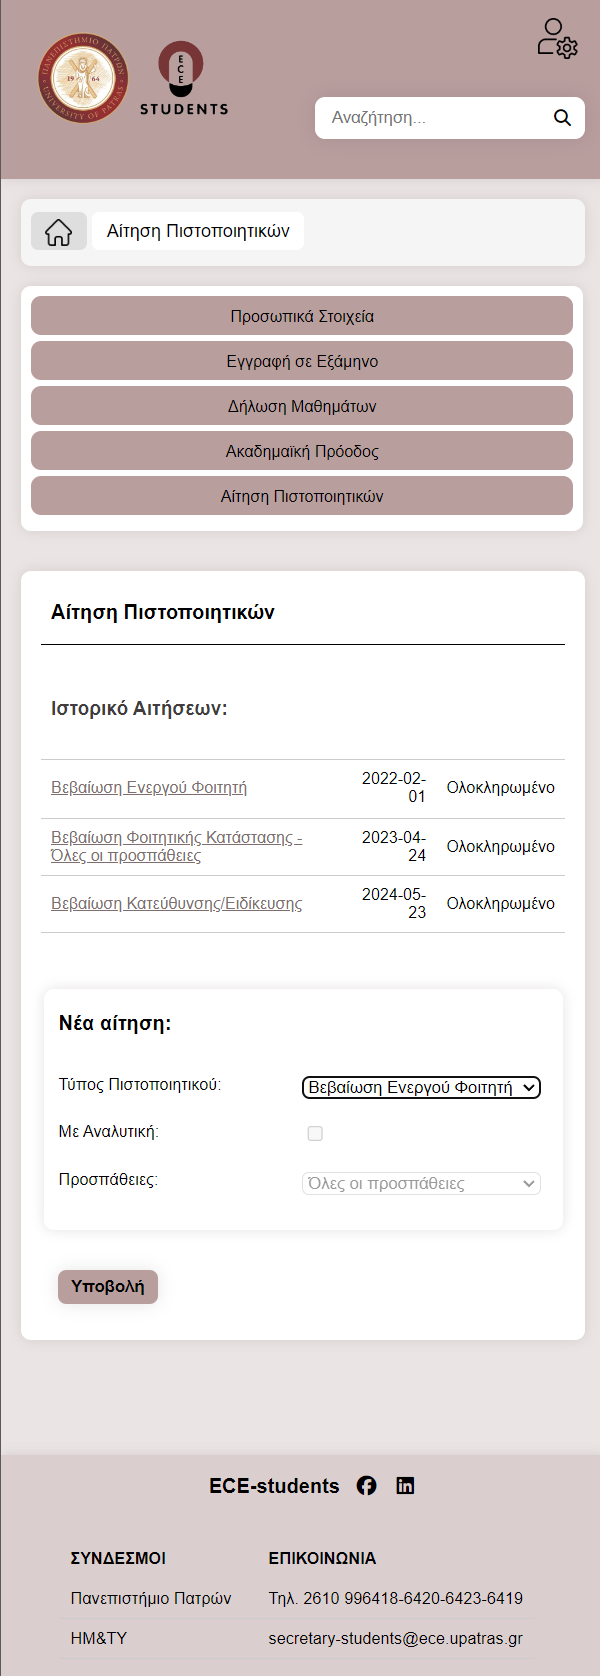
\includegraphics[width=0.3\textwidth]{certificates_mobile.png}
    \caption{\gr{Σελίδα πιστοποιητικών σε} mobile view}
    \label{fig:enter-label}
\end{figure}

\section{\gr{Κώδικας εφαρμογής}}
\gr{Για την οργάνωση του κώδικα χρησιμοποιήθηκε η δομή} MVC (Model, View, Controller).
\\\gr{Η εφαρμογή αποτελείται από τους φακέλους:}
\begin{enumerate}
    \item app-setup \\\gr{Περιλαμβάνει τις συνεδρίες των χρηστών}
    \item controller \\\gr{Περιλαμβάνει αρχεία με τις συναρτήσεις ελέγχου για το} login, \gr{την αυθεντικοποίηση και την λειτουργία των σελίδων της εφαρμογής}
    \item model \\\gr{Περιλαμβάνει την βάση δεδομένων, τα αρχεία δημιουργίας της και το αρχείο σύνδεσης της εφαρμογής με αυτήν}
    \item public \\\gr{Περιλαμβάνει όλες τις εικόνες που χρησιμοποιεί η εφαρμογή και τα αρχεία} CSS \gr{και} JavaScript
    \item routes \\\gr{Περιλαμβάνει τις διαδρομές της ιστοσελίδας}
    \item views \\\gr{Περιλαμβάνει τα αρχεία} handlebars. \gr{Συγκεκριμένα, όλες οι σελίδες της εφαρμογής (εκτός του} login) \gr{χρησιμοποιούν τα ίδια} hbs \gr{αρχεία} header, footer \gr{και} menu \gr{και διαθέτουν} breadcrumb navigation.
\end{enumerate}

\subsection{\gr{Επικοινωνία με τη βάση δεδομένων και με τον server}}
\gr{Χρησιμοποιήσαμε} SQLite3 \gr{για τη βάση δεδομένων μας που δημιουργείται στον φάκελο} model \gr{και συνδέεται με την εφαρμογή μέσω του} student\_services\_lite.mjs . \gr{Αυτό επιτυγχάνεται με μηχανισμό υποσχέσεων} (Promises) \gr{που υποστηρίζει ασύγχρονη εκτέλεση κώδικα. Οι συναρτήσεις του μοντέλου αυτού καλούνται στα αρχεία του} controller \gr{για επικοινωνία με τα αρχεία} handlebars \gr{του φακέλου} views. \gr{Έπειτα, αφού οι σελίδες έχουν αντιστοιχιστεί σε διαδρομές στο αρχείο} routes.mjs, \gr{το αρχείο} server.mjs \gr{καλεί αυτές τις διαδρομές, διαχειρίζεται τα} sessions \gr{και διαθέτει επίσης κάποιες βοηθητικές μεταβλητές} (helpers) \gr{για τα} hbs \gr{αρχεία. Τέλος, το} start.mjs \gr{είναι το αρχείο που καλείται τελικά ώστε η εφαρμογή να λειτουργεί στον δρομολογητή που έχουμε ορίσει.}
\subsection{\gr{Εκκίνηση εφαρμογής}}
\gr{Για να τρέξουμε τοπικά την εφαρμογή ακολουθούμε τα βήματα που περιγράφονται στο αρχείο} \textbf{README.md}.
\\
\\\gr{Ειδικότερα:}
\\
\\\gr{Αφού εγκαταστήσουμε την} Node.js, \gr{τρέχουμε τις εντολές:}
\\\textbf{npm install nodemon -g}
\\\textbf{npm install}
\\
\\\gr{Στη συνέχεια, δημιουργούμε τη βάση δεδομένων, με τις εντολές:}
\\\textbf{pyhton3 database.py}
\\\textbf{python3 fill\_db.py}
\\
\\\gr{Τέλος, για να εκκινήσουμε τον} server \gr{τρέχουμε την εντολή:}
\\\textbf{npm run start}

\subsection{\gr{Κώδικας της εργασίας}}
\gr{Ο κώδικας της εφαρμογής} ECE-Students \gr{μπορεί να βρεθεί στον σύνδεσμο:}
\href{https://github.com/NektariaVer/---------}{GitHub Link}

\end{document}

